\documentclass[11pt]{article}
\usepackage{graphicx,amsmath,amssymb,multirow,xspace}
\usepackage{url}
\parindent0pt
\def\erfinv      {\ensuremath{\mathrm{erf}^{-1}}}
\def\chisq       {\ensuremath{\chi^2}\xspace}
\def\xprime      {\ensuremath{x^{\prime}}\xspace}
\def\xprimesq    {\ensuremath{{x^{\prime}}^2}\xspace}
\def\yprime      {\ensuremath{y^{\prime}}\xspace}
\begin{document}
In the $K\pi$ mixing analysis, we computed confidence contours in 2 dimensions, $n=2$. This was done by computing $-2\Delta\log{\cal L}$, that is, by taking twice the difference in 
$\log$ likelihood between the fit with mixing and another fit where $\xprimesq = \yprime = 0$, but allowing all the other parameters which were allowed to float in  
the standard mixing fit to float here as well. 
It was shown using toy Monte Carlo, that $-2\Delta\log{\cal L}$ was 
distributed like $\chisq$ for $n=2$ degrees of freedom. We would like to construct
regions in parameter space which encompasss the true parameter value with
some probability, called the {\it coverage probability}, $1-\alpha$
\par
The probability $\alpha$ for exceeding \chisq with $n$ degrees of freedom is given by
\begin{equation}
\alpha(\chisq;n) = \left[2^{n/2}\Gamma\left(\frac{n}{2}\right)\right]^{-1}\int_{\chisq}^{\infty}t^{\frac{n}{2}-1}e^{-t/2}dt\label{eq:prob}
\end{equation}
\begin{description}
\item[$n=1$:]
Using $\Gamma(1/2)=\sqrt{\pi}$, Eq.~\ref{eq:prob} becomes:
\begin{equation}
\alpha(\chisq;1) = \frac{1}{\sqrt{2\pi}} \int_{\chisq}^{\infty}
\frac{1}{\sqrt{t}}e^{-t/2}dt\label{eq:probone}
\end{equation}
Using the variable substitution $t/2 = y^2$, Eq.~\ref{eq:probone} becomes
\begin{equation}
\alpha(\chisq;1) = \frac{2}{\sqrt{\pi}}\int_{\sqrt{\frac{\chisq}{2}}}^{\infty}e^{-t}dt=1-\mathrm{erf}\left[\sqrt{\chisq/2}\right]\label{eq:probonep}
\end{equation}
\item[n=2:] Eq.~\ref{eq:prob} becomes:
\begin{equation}
\alpha(\chisq;2) = \frac{1}{2}\int_{\chisq}^{\infty}e^{-t/2}dt=e^{-\chisq/2}\label{eq:probtwo}
\end{equation} 
\end{description}
For higher values of $n$, the following recursion relation can be used:
\begin{equation} 
\alpha(\chisq;n+2) = \alpha(\chisq;n) +\frac{\left[\chisq/2\right]^{n/2}e^{-\chisq/2}}{\Gamma\left(\frac{n}{2}+1\right)}\label{eq:probn} 
\end{equation} 
The difference $-2\Delta\log{\cal L}$ due to statistical errors was determined to be 23.9 units. This was reduced by a factor $1.3$ to 18.4 to account for systematic uncertainties.
This change in log likelihood corresponds to a p-value of 0.00001 for $n=2$. To convert this to ``standard deviations'' we use the following expression
\begin{equation}
1-\alpha = \frac{1}{\sqrt{2\pi}}\int_{-S}^{+S}e^{-y^2/2}dy = \mathrm{erf}\left[{S/\sqrt{2}}\right]\label{eq:Srel}
\end{equation}
Thus,
\begin{equation}
S=\sqrt{2}\erfinv(1-\alpha)\label{eq:S}
\end{equation}
%\begin{figure}[phtb]
%  \centerline{%
%    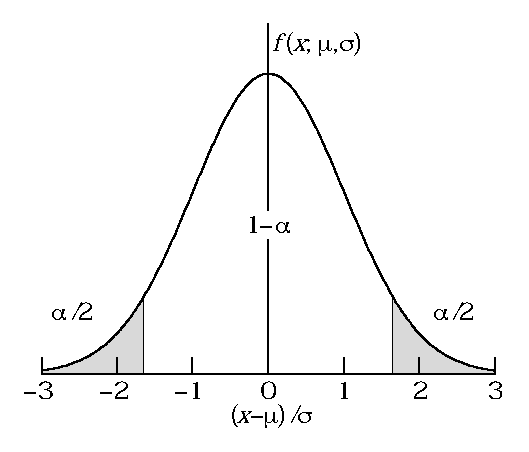
\includegraphics[width=0.6\linewidth, clip=]{std.eps}
%}
%\caption{Illustration of a symmetric 90\% confidence interval (unshaded)
%for a measurement of a single quantity with Gaussian errors. Integrated
%probabilities, defined by $\alpha$, are also shown. The independent variable is
%$S=(x-\mu)/\sigma$.}
%\label{fig:CI}
%\end{figure}
In my opinion, use of this formula to express standard deviations in the 
multivariate case is not internally consistent since this formula gives the 
confidence interval for a measurement of a single quantity with Gaussian
errors. In the multivariate case, one usually quotes the coverage probability
$1-\alpha$ for joint estimation of $n$ parameters. This is simply the 
probability that the given region contains the true values of the parameters.
\par
For particular values of the coverage probability $1-\alpha$, 
Table~\ref{tab:converage} lists the change in log likelihood 
$-2\Delta\log{\cal L}$ for $n=1$ and $n=2$. For $n=1$, the change in log 
likelihood as a function of the coverage probability $1-\alpha$ is given by
\begin{equation}
-2\Delta\log{\cal L}=2\left[\erfinv(1-\alpha)\right]^2
\end{equation}
For $n=2$, the corresponding change in log likelihood is
\begin{equation}
-2\Delta\log{\cal L}=2\log(1-\alpha).
\end{equation}
\begin{table}[ph]
  \begin{center}
  \begin{tabular}{l|c|c}\hline\hline
$1-\alpha$ & $n=1$ & $n=2$ \\ \hline
0.6827  & 1.00 & 2.30 \\
0.9     & 2.71 & 4.61 \\
0.95    & 3.84 & 5.99 \\
0.9545  & 4.00 & 6.18 \\
0.99    & 6.63 & 9.21 \\
0.9973  & 9.00 & 11.83 \\
0.999   & 10.83 & 13.82 \\
0.9999  & 14.14 & 18.42 \\ \hline\hline
\end{tabular}
\label{tab:coverage}
\caption{The change in log likelihood $-2\Delta\log{\cal L}$ 
corresponding to values of the coverage 
probability $1-\alpha$, for joint estimates of $n$ parameters, in the large data sample limit.}
  \end{center}
\end{table}
\end{document}
